\section{Feature Selection}

\begin{frame}
\frametitle{Correlation Analysis}
To determine the most important features in our data, we first of all perform a correlation analysis. The result of the analysis is demonstrated in the figure overleaf. 

From the figure we can see that a lot of parameters are highly correlated with some other features. A very good example of it is the parameter Dew which has 98 percent correlation with the parameter Vapor Pressure.
\end{frame}

\begin{frame}
\frametitle{Correlation Analysis - Result}
\begin{figure}
	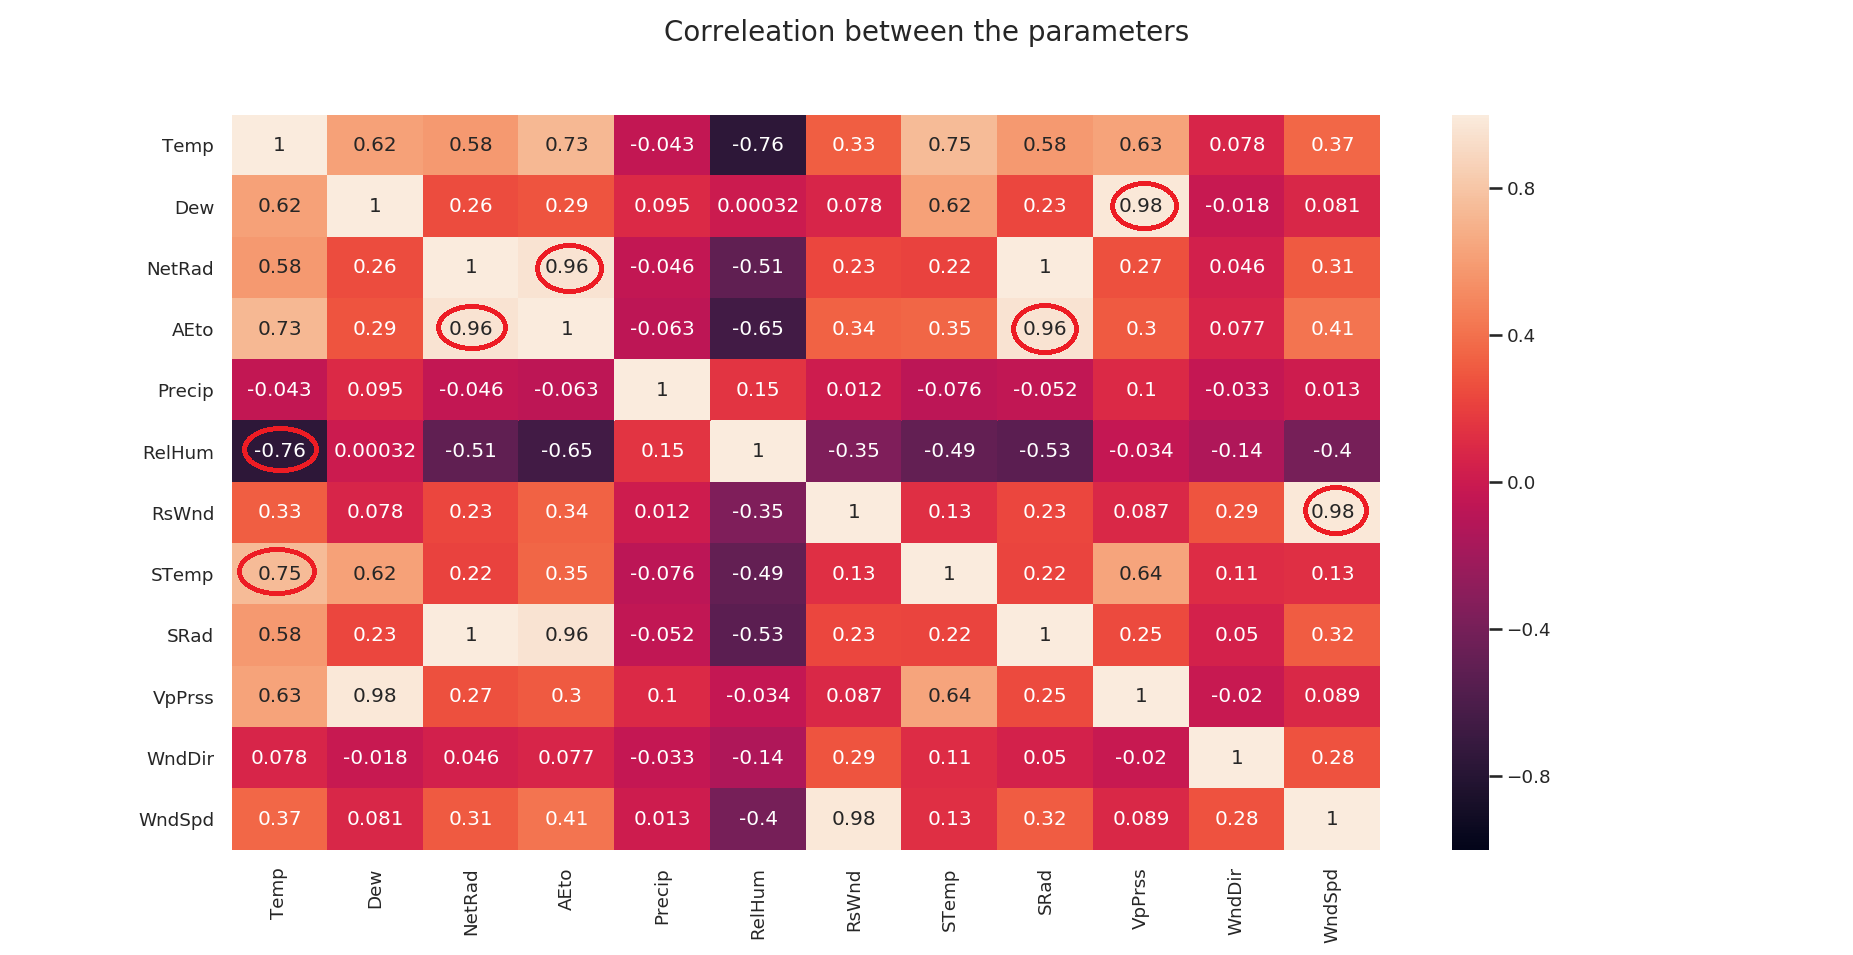
\includegraphics[width=1\textwidth]{images/correleation.png}
\end{figure}
\end{frame}

\begin{frame}
We then visualize the data using first two components of the Principal Component Analysis (PCA). PCA is a commonly used tool that reduces the dimensionality of a dataset by determining the subset of features that captures the highest amount of variance within the data. The biplot diagram overleaf presents the relative "importance" of each of our feature on the over all data(length of each feature line emphasize its importance).


Based on these analysis, we proceed to select 6 most important features namely: Temperature, Radiation, Precipitation, Vapor Pressure, Wind direction and Wind speed.
\end{frame}


\begin{frame}
\frametitle{Biplot-all}
\begin{figure}
	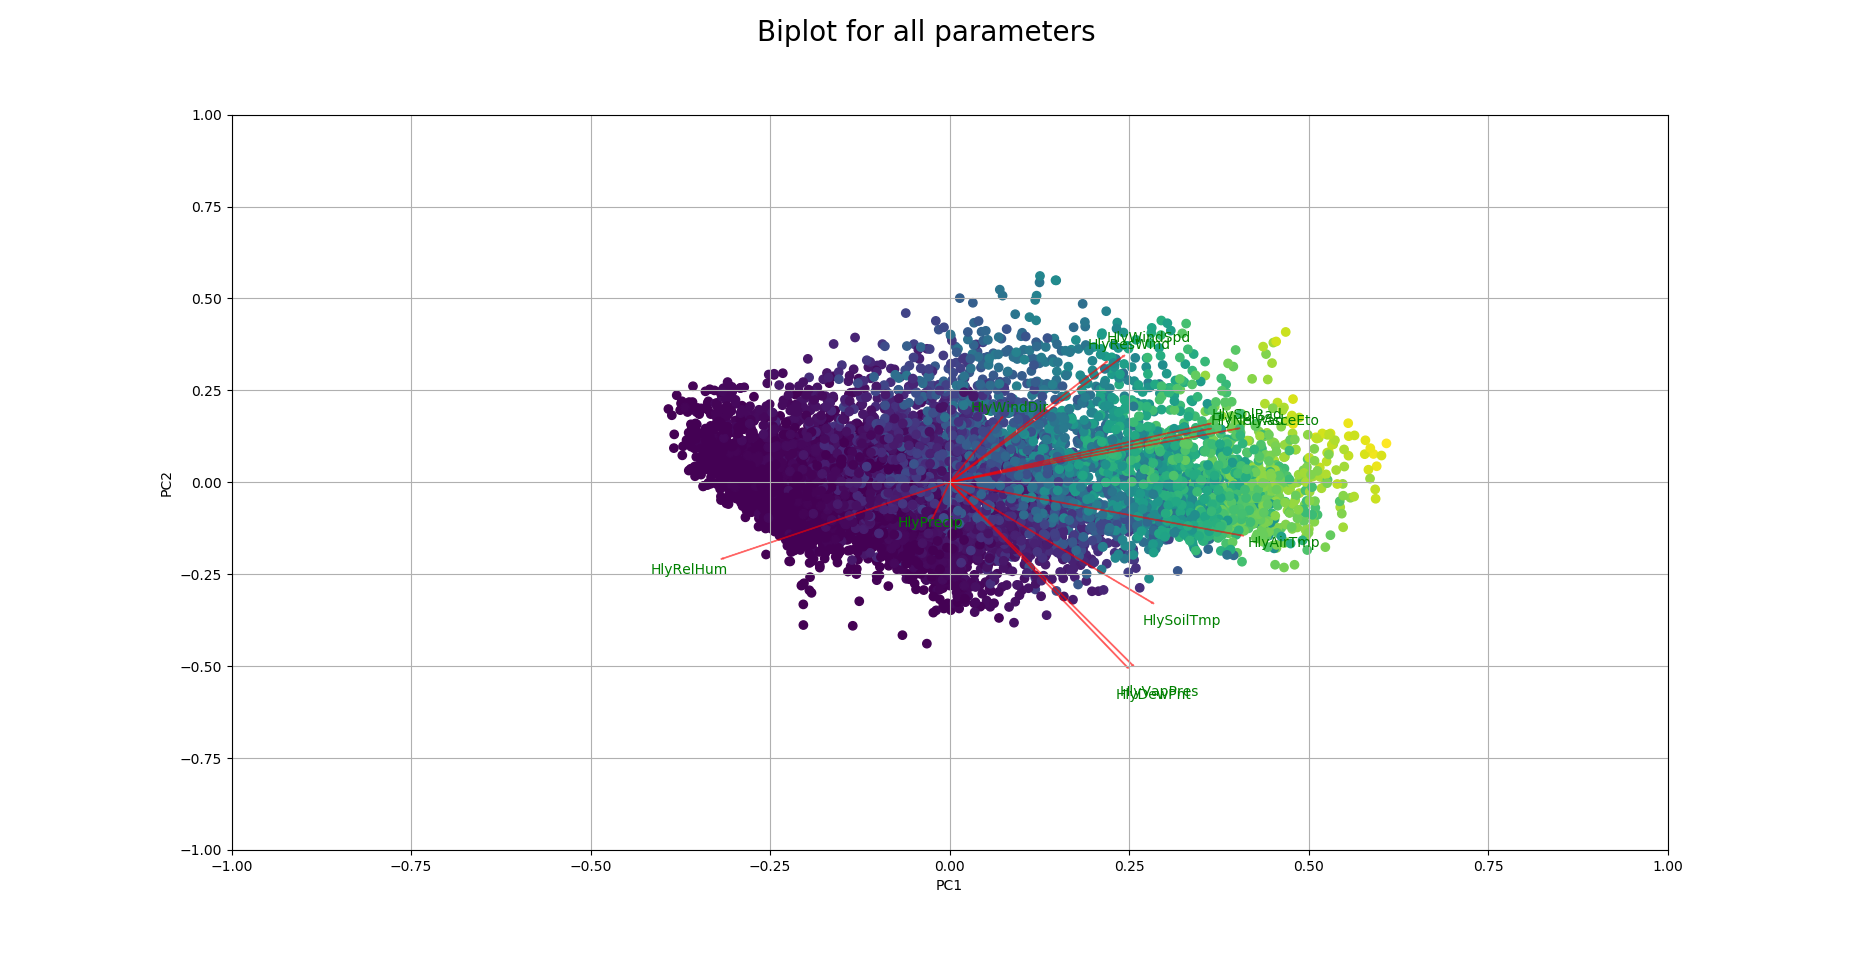
\includegraphics[width=1\textwidth]{images/biplot_full.png}
\end{figure}
\end{frame}


\begin{frame}
\frametitle{Biplot-selected}
Figure below shows the biplot view of the selected features.
\begin{figure}
	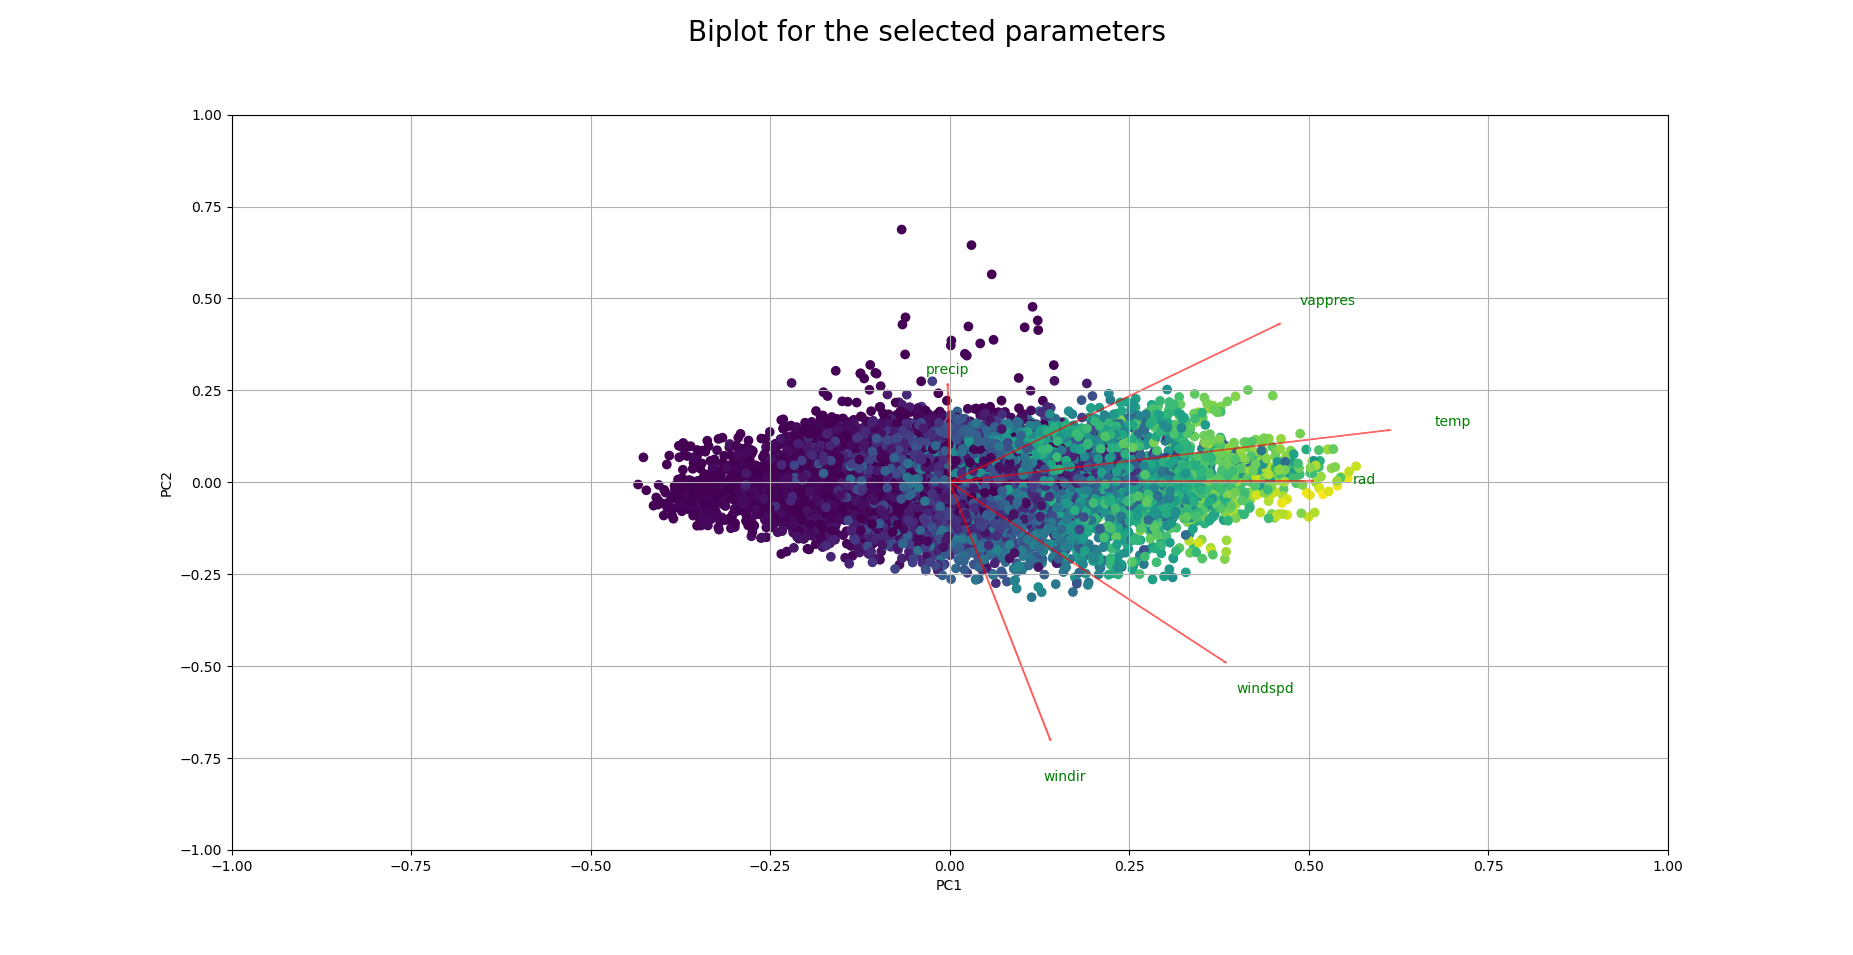
\includegraphics[width=1\textwidth]{images/biplot_selected.png}
\end{figure}
\end{frame}

\begin{frame}
\frametitle{PC1 values}
We finally check the eigenvalues of our selected features on the first principal component eigenvectors. The figure overleaf shows the value each of our parameter possess in this analysis (the values have been multiplied by 10.)

Based on these values, for the rest of our analysis for this project, we use the features, Temperature, Radiation, Vapor Pressure and Wind Speed (the four most important parameters according to PCA.)
\end{frame}


\begin{frame}
\frametitle{PC1 values}
\begin{figure}
	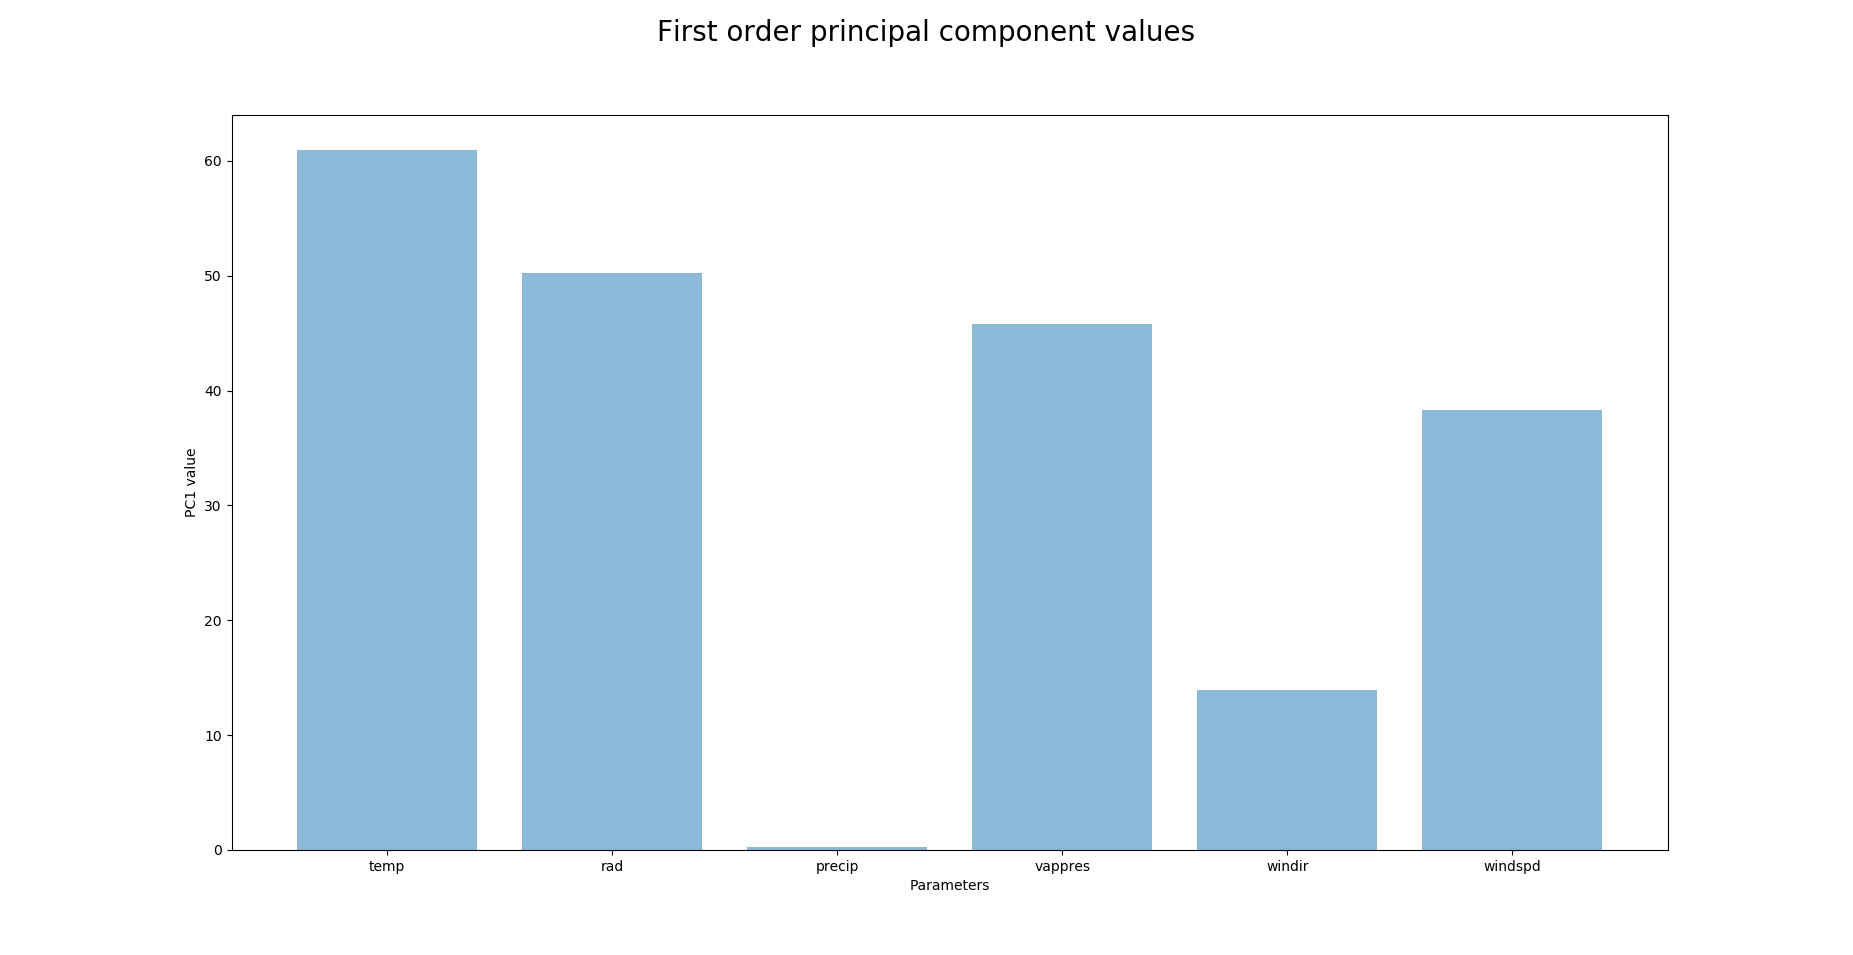
\includegraphics[width=1\textwidth]{images/PC1_values.png}
\end{figure}
\end{frame}